\JWlone{Design}
\label{sec:design}


%#  BIG PICTURE  ###############################################################
\JWltwo{Big Picture of the Setup}
\label{sec:big-pic}

\begin{figure}
  \centering
    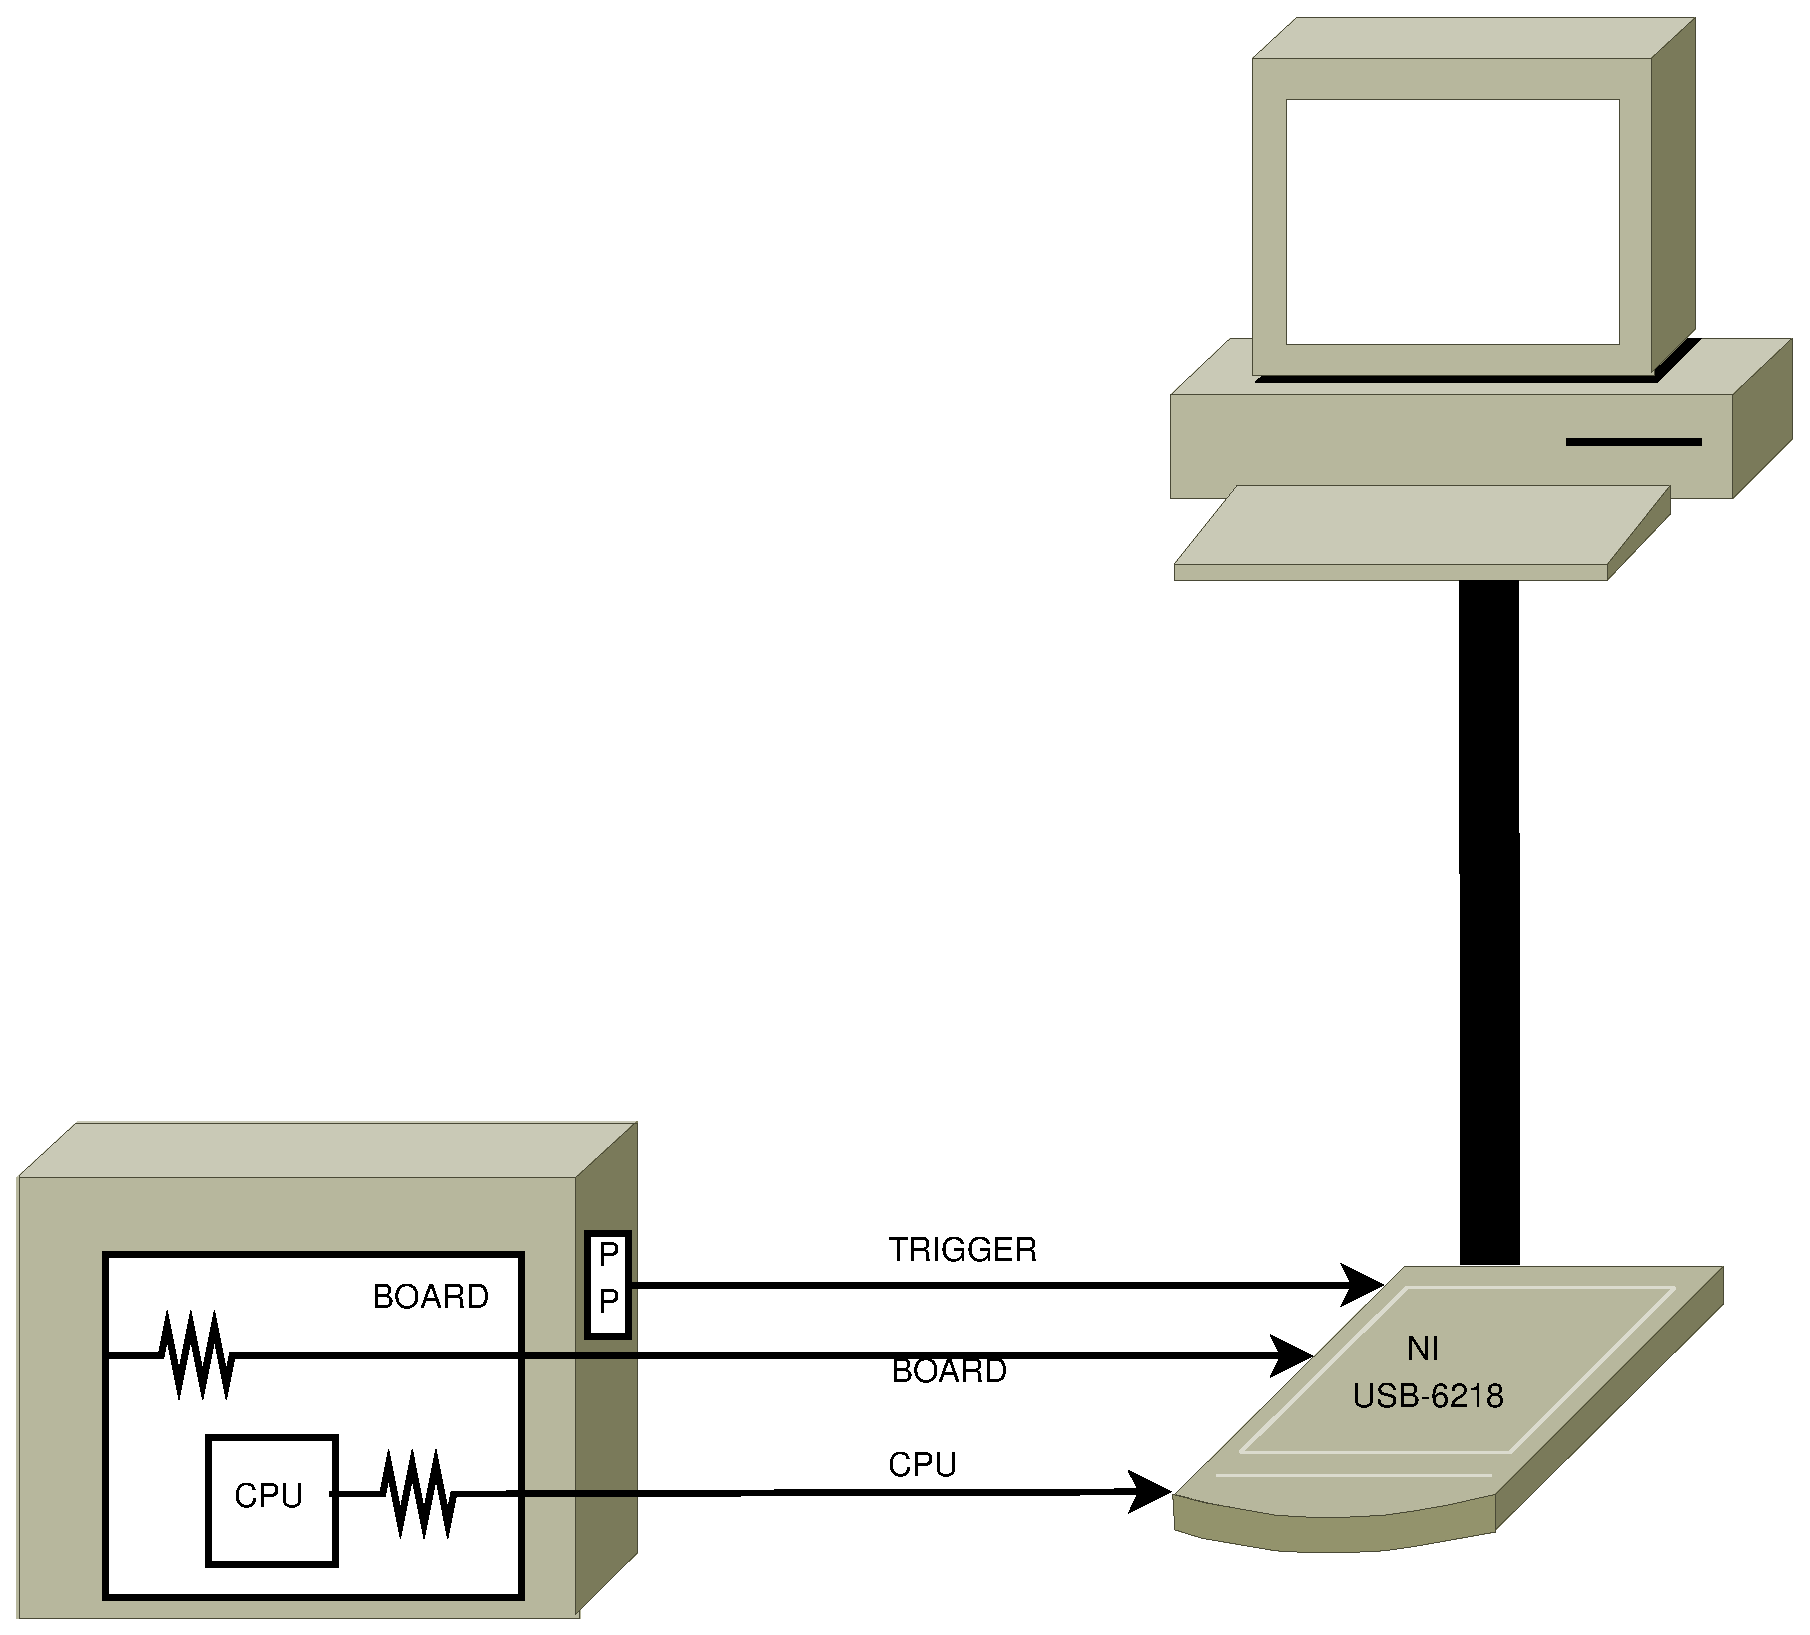
\includegraphics[width=\textwidth]{fig/measuring-overview.eps}
  \caption{Measuring setup overview}
  \label{fig:overview}
\end{figure}

As figure \ref{fig:overview} illustrates an additional workstation---the
\emph{Examining Workstation (EW)}---has been used while evolving this thesis.
The \emph{System under Test (SuT)} counts the CPU's performance events itself
and the EW records the energy consumption using a measuring device in the
meantime. These two data sets have thereafter been used to build up the energy
model.


%#  MEASURING SETUP IN DETAIL  #################################################
\JWltwo{Measuring Setup in Detail}
\label{sec:measuring-setup}

To fit the energy model later, the current flows of the CPU and the
motherboard's \SI{12}{\volt} supply have to be measured. Using four--terminal
sensing \cite{wiki:FTS} voltage drops across the sensing resistor are
measured to deduce the current flow. The motherboard's \SI{12}{\volt} current
flow has been measured in this thesis because it was unclear if the CPU is
entirely fed by its own \SI{12}{\volt} power supply.

Because the SuT and the EW (see figure \ref{fig:overview}) have to agree about
the examination (time) interval a trigger wire is used. It is realized as a
simple analog signal using the parallel port's \emph{high} and \emph{low}
voltages.

This can be summed up to measure three potential differences. Since the
measuring device (chapter \ref{sec:measuring-device}) provides up to eight
differential, analog input channels this seems easy at first. Unfortunately,
two caveats apply: On the one hand according to the user's manual
\cite{NIManual2009} the best measuring accuracy can be achieved in range of
\SI{-200}{\milli\volt} and \SI{200}{\milli\volt}. On the other hand the overall
potential differences may not exceed $\pm$\SI{10.4}{\volt} \cite{NISpec2009}.

\begin{figure}
  \centering
    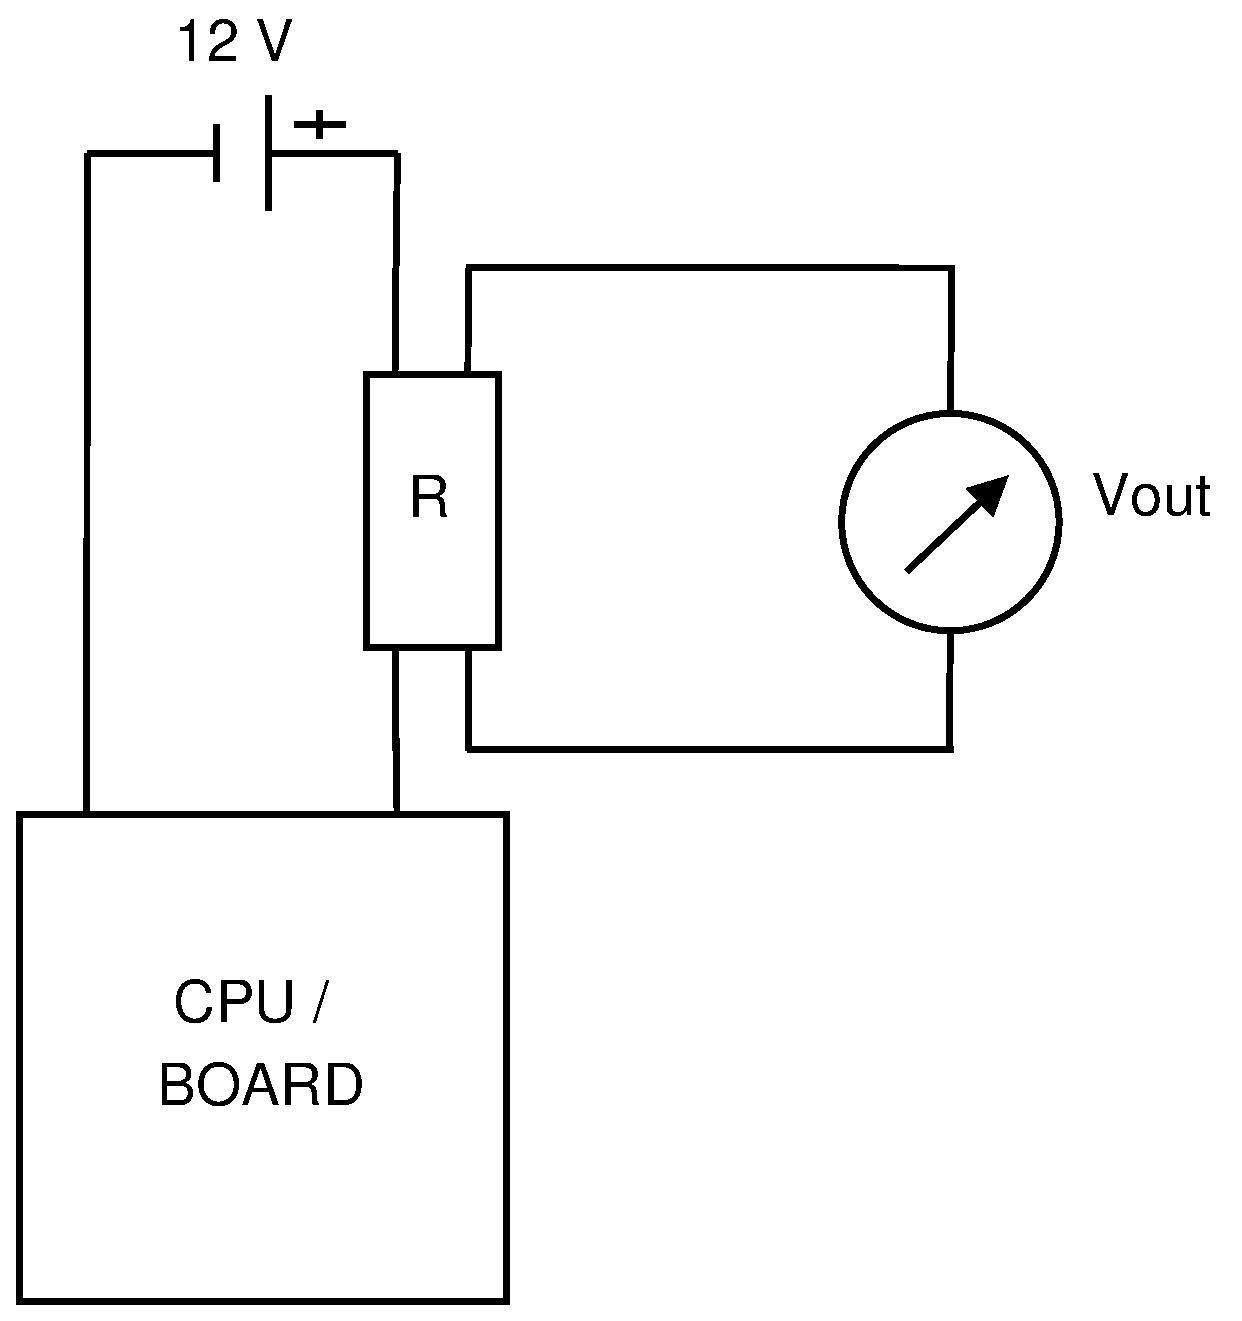
\includegraphics[width=0.5\textwidth]{fig/measuring-circuit.eps}
  \caption{Measuring circuit for CPU (R=\SI{10}{\milli\ohm}) and BOARD
(R=\SI{5}{\milli\ohm})}
  \label{fig:circuit}
\end{figure}

\begin{figure}
  \centering
    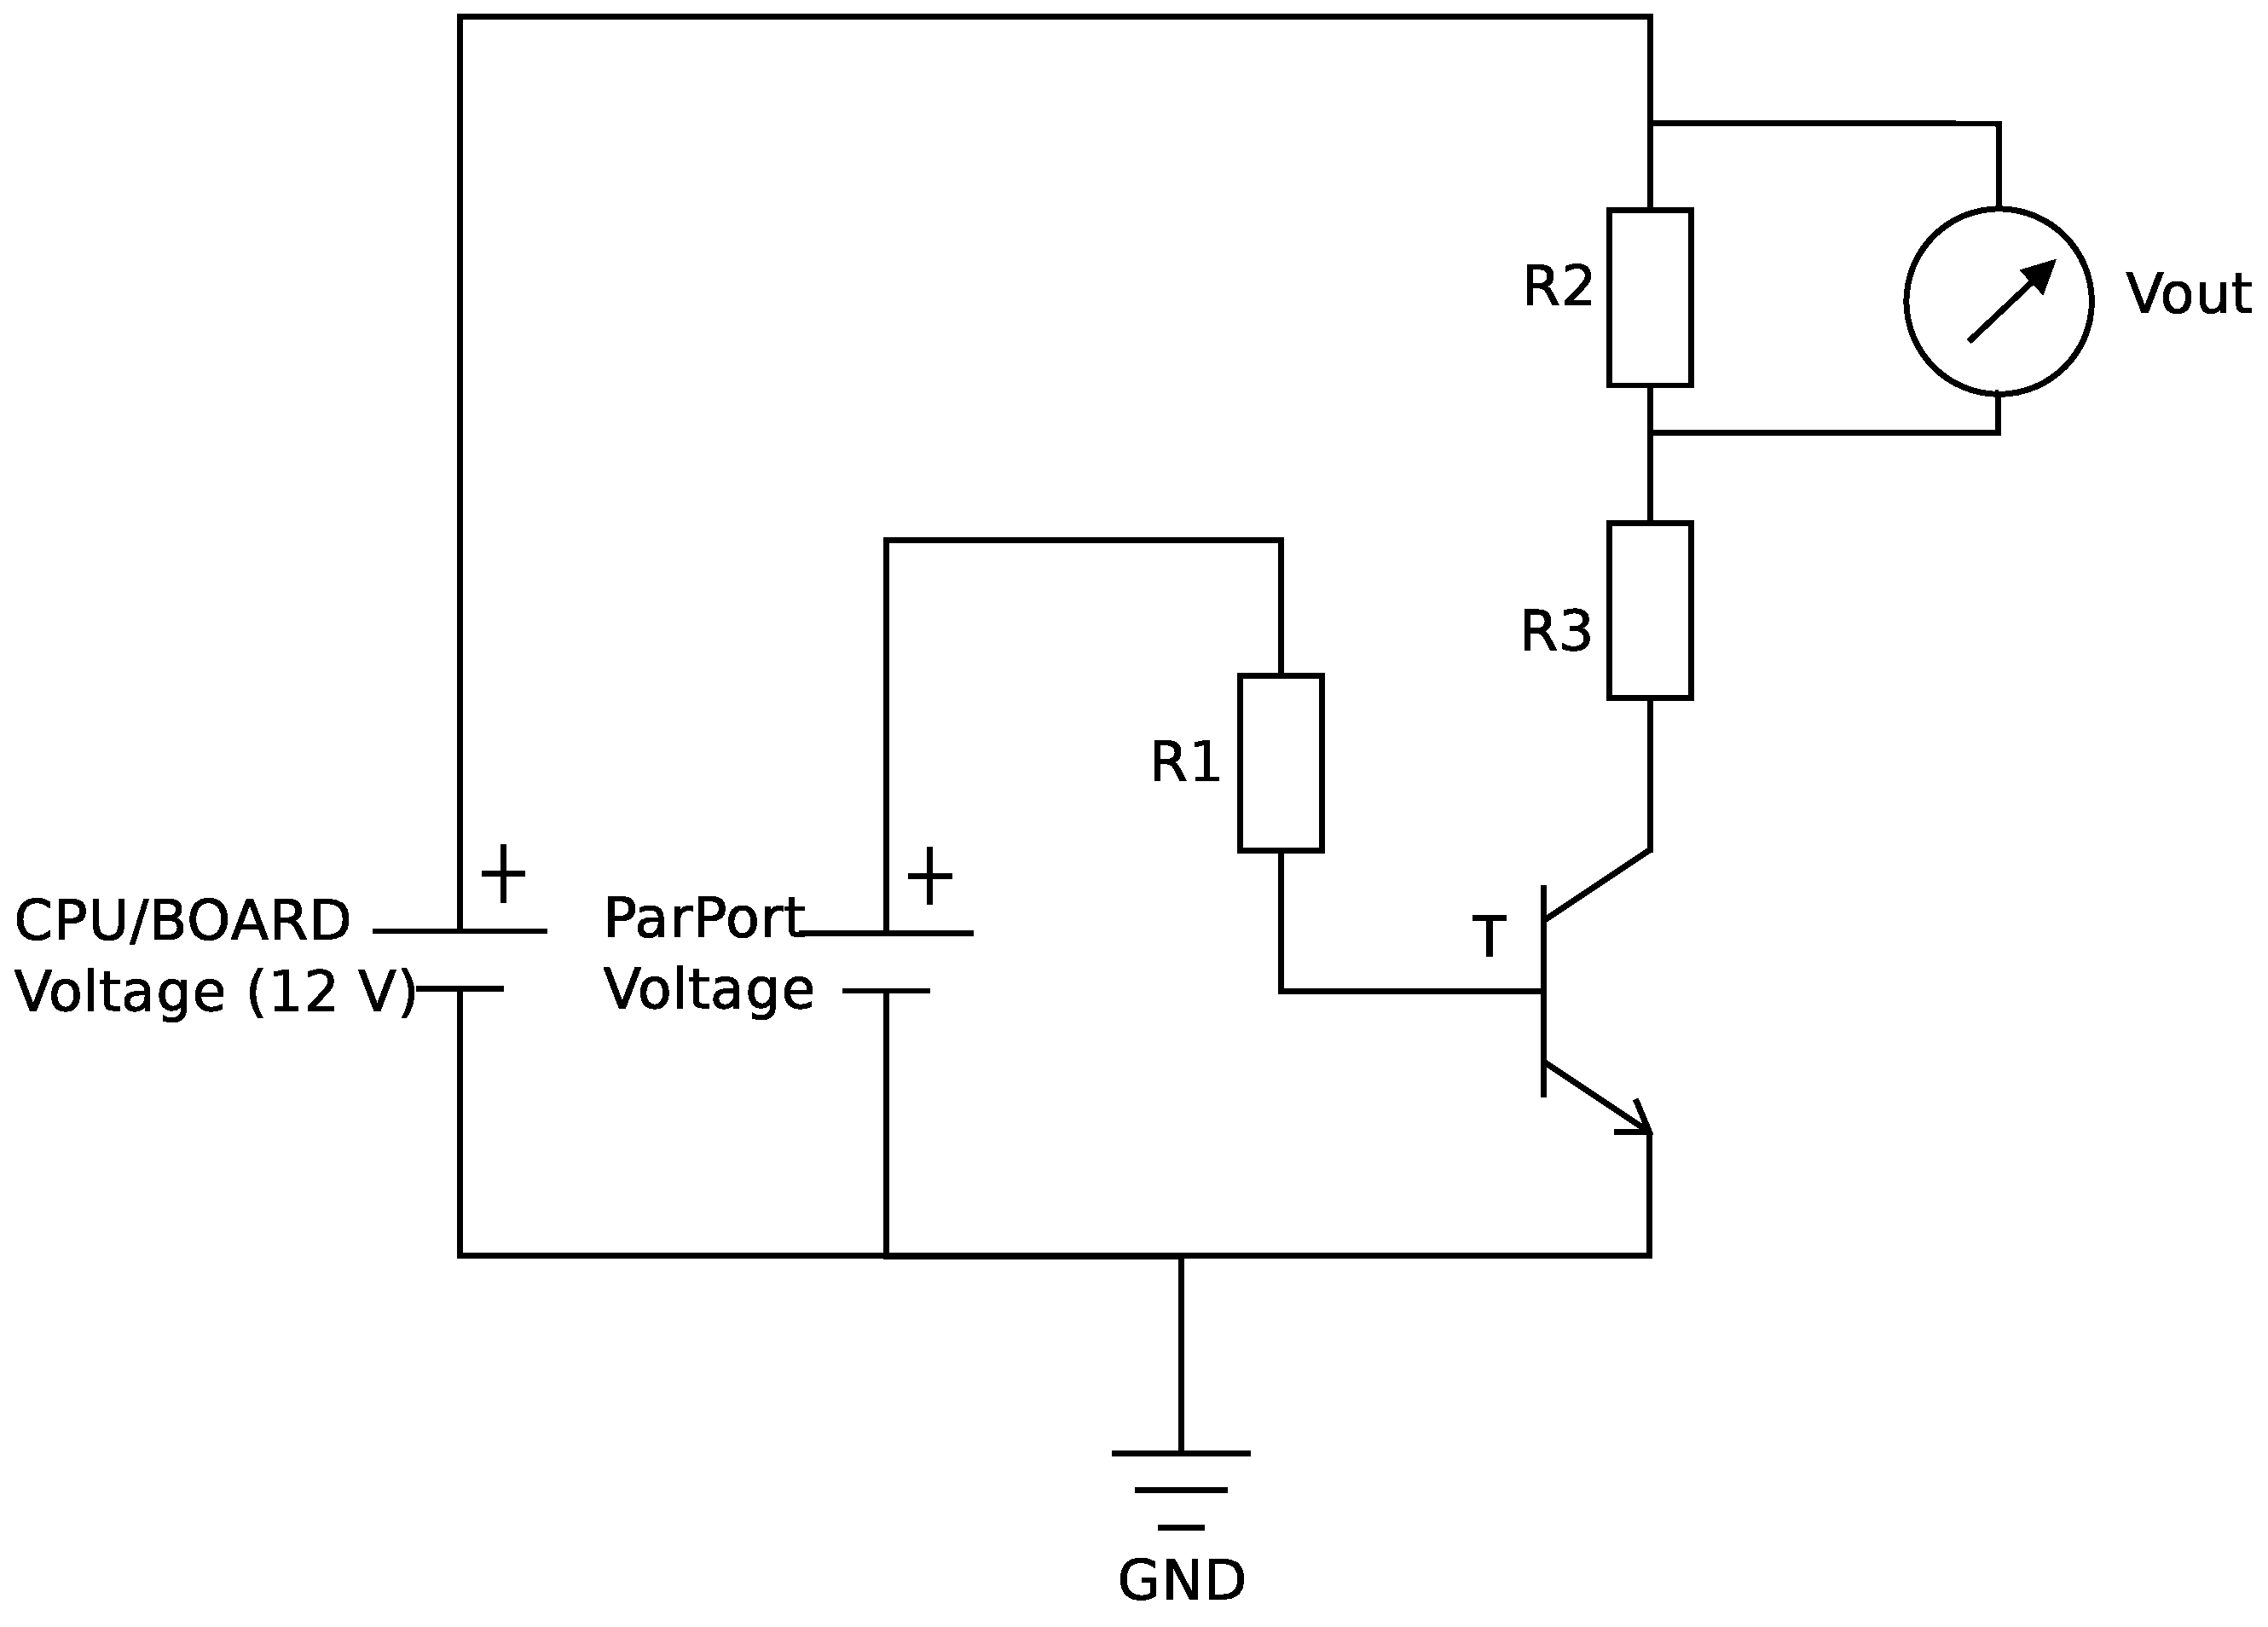
\includegraphics[width=\textwidth]{fig/potential-equalizer.eps}
  \caption{Potential equalizer}
  \label{fig:potential-equalizer}
\end{figure}

Choosing adequate sensing resistors for the \JWchan{CPU} (R =
\SI{10}{\milli\ohm}) and \JWchan{BOARD} (R = \SI{5}{\milli\ohm}) channels (see
figure \ref{fig:circuit}) worked out well. The parallel port trigger wire has
been a problem at first, though. The parallel port has a potential difference
range of more than \SI{200}{\milli\volt} and our test machine's port had a very
different potential level than the \JWchan{CPU} and \JWchan{BOARD} channels,
exceeding the allowed range of $\pm$\SI{10.4}{\volt}.  The potential equalizer
illustrated in figure \ref{fig:potential-equalizer} solves both problems.

Finally, three differential channels \JWchan{CPU}, \JWchan{BOARD}
(\SI{12}{\volt} supply only!) and \JWchan{TRIGGER} in the range of
$\pm$\SI{200}{\milli\volt} and alike potential levels can be connected to the
measuring device. The performance events get counted on the SuT itself which
controls the trigger wire, too: The trigger is set to \emph{On} directly before
executing the program to examine and is set to \emph{Off} promptly after its
termination. To safely register all CPU energy consumption peaks, a high
sampling rate of \SI{50}{\kilo\samples\per\second} is chosen. An exemplary
plot of an examination can be found in figure \ref{fig:cpu-power-trig}.

\begin{figure}
  \centering
    \includegraphics[width=\textwidth]{fig/cpu-power-trig.eps}
  \caption{Sample examination}
  \label{fig:cpu-power-trig}
\end{figure}

\JWtodo{Bild, auf dem man den Timer-Interrupt sieht}


%-  measuring device  ----------------------------------------------------------
\JWlthree{Measuring Device}
\label{sec:measuring-device}

For measuring the voltage drops \JWPLni{} from
\JWenterprise{http://www.ni.com}{National Instruments} (shown in figure
\ref{fig:ni}) was chosen because it supports high sampling rates of up to 250000
samples per second (\SI{250}{\kilo\samples\per\second}) and is very accurate
(accuracy $< \SI{2.69}{\milli\volt}$)\cite{NISpec2009}.

\begin{figure}
  \centering
    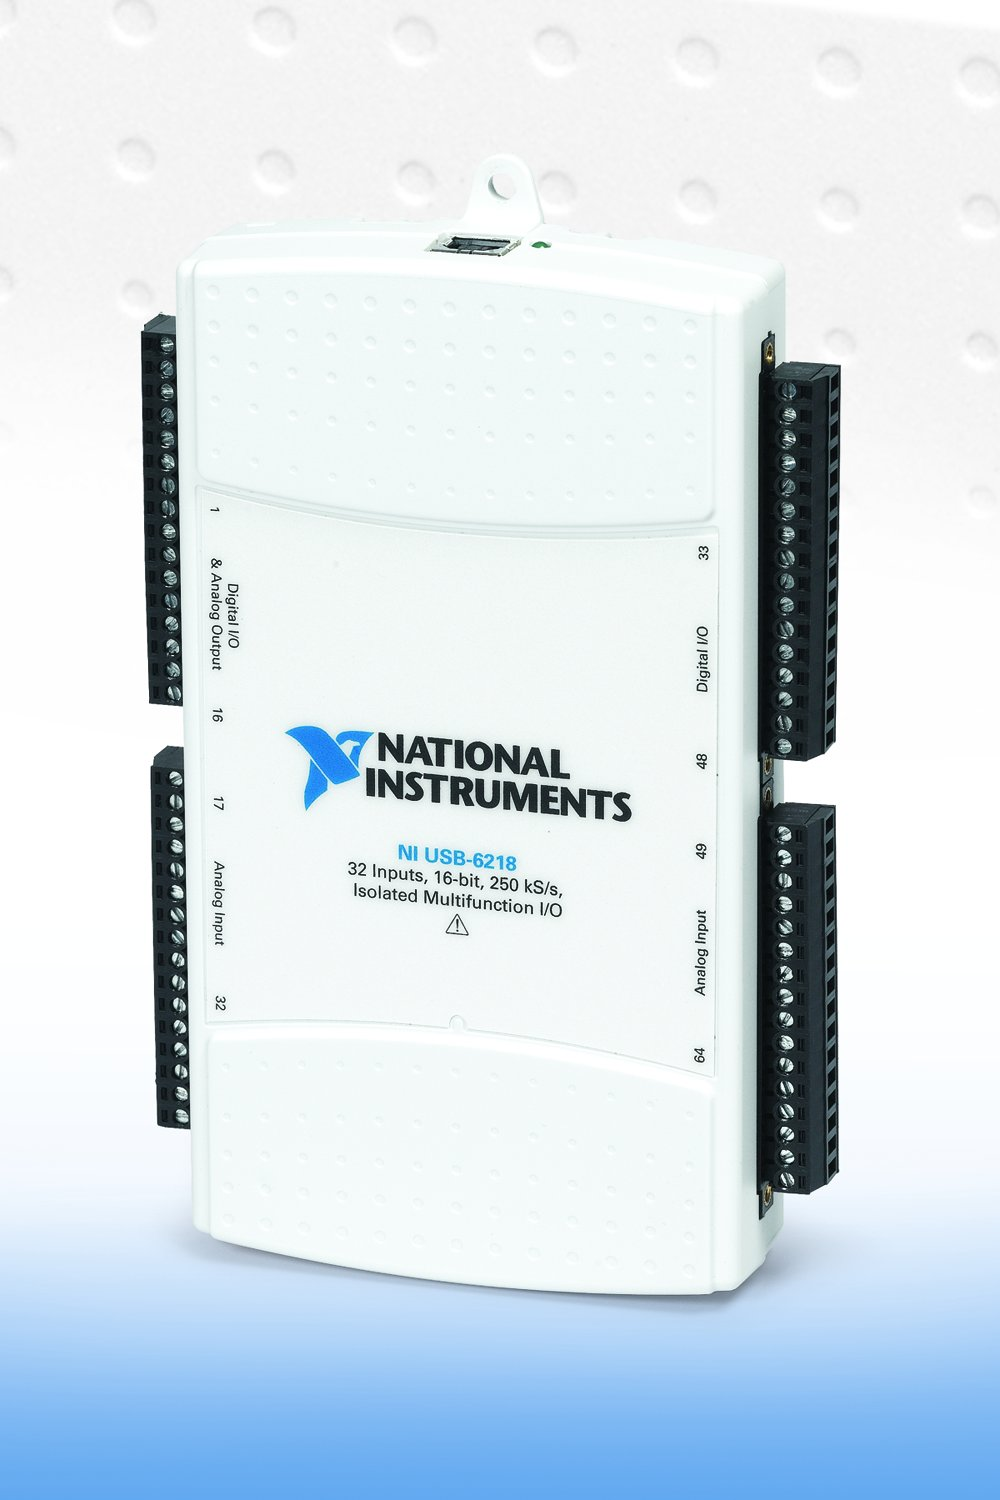
\includegraphics[width=0.5\textwidth]{fig/NI-USB-6218.jpg}
  \caption{\JWPni{} (picture from \JWlink{http://www.pressebox.de/pressemeldungen/national-instruments-germany-gmbh/boxid/75241})}
  \label{fig:ni}
\end{figure}


%#  CALCULATION OF THE ELECTRICAL WORK  ########################################
\JWltwo{Calculation of the Electrical Work}
\label{sec:calc-work}

From elementary physics

\begin{eqnarray}
     U_R & = & R * I \\
  \iff I & = & \frac{U_R}{R}
\end{eqnarray}

and

\begin{equation}
  U_{CPU} + U_{R} = 12 V
\end{equation}

we obtain the instantaneous power of the CPU by measuring the voltage drop
across the sensing resistor:

\begin{eqnarray}
P_{CPU}(t) & = & (12V - U_R(t)) * \frac{U_R(t)}{R} \\
           & = & \frac{12V * U_R - {U_R}^2}{R} \\
           & \stackrel{0 < U_R \ll 1}{\approx} & \frac{12V * U_R}{R}.
\end{eqnarray}

Hence, integrating will result in the electrical work

\begin{equation}
  W = \int P_{CPU}(t)dt.
\end{equation}


%#  ENERGY MODEL  ##############################################################
\JWltwo{Energy Model}
\label{sec:model}

The following chapters will define the term \emph{energy model} along with  the
formal methods suggested to build such a model.


%-  the model's properties  ----------------------------------------------------
\JWlthree{Properties}
\label{sec:model-properties}

In this work, an energy model is considered as a linear formula. A system with
$n_c$ cores that is able to monitor $n_e$ performance events per core
simultaneously is described. Additionally to the per--core event counters, $n_g$
global event counters make the model up. In the formal description (see chapter
\ref{sec:towards-the-model} for the practical implementation) we assume four
functions providing the actual values:

\begin{itemize}

\item $c_g(i, t_0, t_e)$, the global event $i$'s count in the time interval
$(t_0, t_e)$

\item $c_e(j, k, t_0, t_e)$ the performance event $k$'s count on core $j$ in the
interval $(t_0, t_e)$

\item $w_g(i)$ the global event $i$'s energy weight in \si{\joule}

\item $w_e(j, k)$ the weight of performance event $k$ in \si{\joule} on core
$j$

\end{itemize}

Though, an energy model equates to

\begin{equation}
W(t_0, t_e) = \sum\limits_{i=1}^{n_g} c_g(i, t_0, t_e) w_g(i) +
\sum\limits_{j=1}^{n_c} \sum\limits_{k=1}^{n_e} c_e(j, k, t_0, t_e) w_e(j, k)
\end{equation}

The functions $c_e$ and $c_g$ contain the system's life data whereas the energy
weights $w_e$ and $w_c$ can be calculated a priori as done in this work.
Obviously the selection of the events and their respective weights highly depend
on the type of microprocessor. To calculate the electrical power the system
consumes, one typically chooses an arbitrary frequency $T$ and sets
the variables $t_0$ and $t_e$ accordingly ($t_0 = ?$, $t_e = t_0 + \frac{1}{T}$)
. The instantaneous power of the instant $t$ is then calculated as:

\begin{eqnarray}
P(t) & = & \frac{W(t - \frac{1}{T}, t)}{\frac{1}{T}} \\
     & = & \frac{\sum\limits_{i=1}^{n_g} c_g(i, t - \frac{1}{T}, t) w_g(i) +
                 \sum\limits_{j=1}^{n_c}
                 \sum\limits_{k=1}^{n_e} c_e(j, k, t - \frac{1}{T}, t) w_e(j, k)
                }{\frac{1}{T}}
\end{eqnarray}

%o_{t_0}(i)
%o_{t_e}(i)

\[
Cg_{n_o,n_g} =
\begin{pmatrix}
c_g(1, b_1, e_1)         & \cdots & c_g(n_g, b_1, e_1)        \\
\vdots                   & \ddots & \vdots                    \\
c_g(1, b_{n_o}, e_{n_o}) & \cdots & c_g(n_g, b_{n_o}, e_{n_o})
\end{pmatrix}
\]

\[
Cc_{n_o,n_cn_e} =
\begin{pmatrix}
c_e(1, 1, b_1, e_1)         & \cdots & c_e(n_c, n_e, b_1, e_1)         \\
\vdots                      & \cdots & \vdots                          \\
c_e(1, 1, b_{n_o}, e_{n_o}) & \cdots & c_e(n_c, n_e, b_{n_o}, e_{n_o})
\end{pmatrix}
\]

\[
C_{n_o,n_g+n_cn_e} = \Bigg( Cg \| Cc \Bigg) =
\begin{pmatrix}
Cg_{1,1}   & \cdots & Cg_{1,n_g}   & Cc{1,1}   & \cdots & Cc{1,n_cn_e} \\
\vdots     & \ddots & \vdots       & \vdots    & \ddots & \vdots       \\
Cg_{n_o,1} & \cdots & Cg_{n_o,n_g} & Cc{n_o,1} & \cdots & Cc{n_o,n_cn_e} \\
\end{pmatrix}
\]

\
\[
w =
\begin{pmatrix}
w_g(1) \\
\vdots \\
w_g(n_g) \\
w_e(1, 1) \\
\vdots \\
w_e(n_c, n_e)
\end{pmatrix}
, j =
\begin{pmatrix}
j_1 \\
\vdots \\
j_{n_o}
\end{pmatrix}
, \epsilon =
\begin{pmatrix}
\epsilon_1 \\
\vdots \\
\epsilon_{n_o}
\end{pmatrix}
\]

\begin{equation}
e = C w + \epsilon
\end{equation}

%-  minimizing the counter set  ------------------------------------------------
\JWlthree{Minimizing the Set of Performance Events}
\label{sec:min-events}

Having seen what exactly constitutes an energy model (chapter
\ref{sec:model-properties}), it is crucial to find a small and significant set
of performance events to use. It is not practical to take into account all
events the microprocessor is aware of. Today's processors offer a lot more
events then they can count simultaneously \cite{intel2011softdev1}.

The approach to find a reasonable subset of $n_e$ events (of $a$ available)
used in this work can be summed up to:

\begin{enumerate}

\item Generation of the matrix of performance event counters $C$ and
the corresponding vector of electrical works $W$

\item Obtaining $C'$ containing the $N$ most correlating columns of $C$

\end{enumerate}

Thereafter, the system of linear equations

\begin{equation}
W = C' * X
\end{equation}

can be solved by simple linear regression.


\JWlfour{Step 1: Generating $C$ and $W$}

\begin{enumerate}[(a)]

\item Choose $p$ test programs which use the CPU differently. The test
programs have to be independent from external events. We consider subsequent
runs of a test program as equal.

\item Divide the $A$ available events in $g$ disjoint, non--empty sets
$E_{1..g}$ of size up to $N$.

\item For each set $E_{1..g}$, run all the $p$ test programs and record the
electrical work and the event counters of the set's events.

\item The electrical work of each of the runs of a test program should be
roughly equal.

\item Folding all the results leads to a vector $W_{1..p}$ containing the
electrical work a run of each of the test programs consumes. Additionally, a
matrix $C = [c_{1..p,1..N}]$ arises, containing each event counter's value for a
run of each of the test programs.

\end{enumerate}

\JWlfour{Step 2: Deriving $C'$ from $C$}

\begin{enumerate}[(a)]

\item Add all columns from $C$ to $C'$

\item Eliminate duplicate columns in $C'$

\item Eliminate columns which contain only zeroes in $C'$

\item Eliminate linear dependent columns in $C'$

\item \JWtodo{weiter}

\end{enumerate}

% vim: set spell spelllang=en_us fileencoding=utf8 : syntax spell toplevel :
